\documentclass[11pt, a4paper]{article}
\usepackage[utf8]{inputenc}
\usepackage{amsmath, amssymb}
\usepackage{graphicx}
\usepackage{booktabs}
\usepackage{tabularx}
\usepackage[margin=1in]{geometry}
\usepackage[dvipsnames]{xcolor}
\usepackage[hidelinks]{hyperref}
\usepackage{url}
\usepackage{float}
\usepackage[font=small, labelfont=bf, skip=6pt]{caption}
\usepackage{enumitem}
\usepackage{microtype}
\setlist{itemsep=2pt, topsep=4pt}

% ---------- colours (match the figures) ----------
\definecolor{navy}{HTML}{4C1D95}
\definecolor{teal}{HTML}{10B981}
\definecolor{brick}{HTML}{EA580C}
\definecolor{greyblue}{HTML}{94A3B8}

% ---------- figure helper: shows a placeholder box if the file is missing ----------
\newcommand{\placefig}[2][\linewidth]{%
  \IfFileExists{#2}{\includegraphics[width=#1]{#2}}{%
    \fbox{\parbox[c][5cm][c]{#1}{\centering\small\textit{Figure placeholder}\\[2pt]\texttt{\detokenize{#2}}}}}}

% ---------- PDF metadata ----------
\hypersetup{
  pdftitle={E-Commerce Behavioral Analytics: Cart Abandonment and User Journey Analysis},
  pdfauthor={Arth Dubey},
  pdfsubject={Measuring cart abandonment, diagnosing its behavioural drivers and prioritising product fixes},
  pdfkeywords={cart abandonment, user journey, HEART, cohort analysis, root-cause analysis, Welch t-test, JTBD, RICE}
}

\begin{document}

% =====================================================================
% Title block
% =====================================================================
\thispagestyle{plain}
\begin{center}
{\small\scshape\color{brick} Project Report }\\[8pt]
{\color{black}\rule{\linewidth}{1.2pt}}\\[14pt]
{\LARGE\bfseries\color{black} E-Commerce Behavioral Analytics:\\[4pt] Cart Abandonment and the User Journey\par}
\vspace{10pt}
{\large\itshape\color{black!75} Measuring Abandonment, Diagnosing Its Behavioural Drivers and Prioritising Product Fixes\par}
\vspace{12pt}
{\color{black}\rule{\linewidth}{0.4pt}}\\[14pt]
{\large\bfseries Arth Dubey\par}
\vspace{3pt}
{\normalsize Indian Institute of Technology Gandhinagar\par}
\vspace{3pt}
{\normalsize\color{black!70} April 2026\par}
\end{center}

\vspace{14pt}

% =====================================================================
% Abstract
% =====================================================================
\noindent{\setlength{\fboxsep}{10pt}\colorbox{black!6}{%
\parbox{\dimexpr\linewidth-2\fboxsep\relax}{%
{\centering\bfseries\color{black} Abstract\par}
\vspace{6pt}
\small
Shoppers put far more into their carts than they buy, and the reasons are rarely obvious. This project analyses 9.0 million real e-commerce events from 46,673 purchasing customers to measure cart abandonment, map how shoppers move through the store, and find what separates heavy abandoners from everyone else. Of 450,463 items added to a cart, 56.7\% were never bought (40.5\% removed, 16.2\% left unresolved), a figure that holds after correcting for items carted near the end of the data window. The metrics were framed with Google's HEART framework, using behavioural proxies for Happiness and Adoption, and the journey was mapped as a transition matrix between event types. Segmenting users by how much of their cart they remove, and testing with Welch's t-test, shows that high-abandon users search 18.9 times more than low-abandon users ($p < 0.001$). A stress test then shows most of that gap comes from comparing active cart users with people who rarely use the cart: among comparable cart users the gap is 2.3 times, and 1.1--1.5 times per session. The more direct evidence for comparison shopping is that one in five abandoned items was followed within a week by the purchase of a different product from the same category. Price was ruled out as a driver (correlation 0.03). Using Jobs-to-be-Done and RICE, a comparison-shopping experience for heavy searchers ranked as the top intervention.

\vspace{6pt}
\noindent\textbf{Keywords:} cart abandonment, user journey, HEART framework, cohort analysis, root-cause analysis, Welch's t-test, JTBD, RICE prioritisation
}}}

\vspace{10pt}

% =====================================================================
\section{Introduction}
Cart abandonment is one of the most studied and least understood problems in online retail. Industry benchmarks put the average rate at around 70\%~\cite{baymard}, but a single rate says nothing about \emph{why} shoppers leave items behind, and different causes call for very different fixes. If shoppers abandon because prices are too high, the answer is pricing. If they abandon because they are comparing options, the answer is to make comparing easier. Discounting a shopper who was going to buy a competing product anyway only gives away margin.

This project works through that diagnosis end to end on real behavioural data, and is organised around four questions:
\begin{enumerate}[label=\textbf{Q\arabic*.}]
  \item How do shoppers move through the store, and where do carted items drop out?
  \item How large is cart abandonment, and is it stable across customer cohorts?
  \item What distinguishes users who abandon heavily, and does the difference survive a fair comparison?
  \item Which product intervention should be built first?
\end{enumerate}
The same questions apply directly to quick commerce and food delivery, where a large share of sessions end with a filled cart that never becomes an order, and where knowing whether a shopper left to compare, to wait or because of price determines what the product should change.

% =====================================================================
\section{Data and Preprocessing}
\subsection{Dataset}
The analysis uses the Synerise RecSys Challenge 2025 dataset~\cite{synerise}: anonymised, real-world interaction logs from an online store, covering page visits, search queries, cart additions and removals, and purchases. Product prices are given as anonymised buckets (0--99), categories as anonymised IDs, and search queries as numerical embeddings rather than text. The full dataset is about 1.9~GB, so a client-level sample was drawn: users were sampled from the purchase log, and every event for those users was kept so that complete journeys stay intact. Table~\ref{tab:data} summarises the sample.

\begin{table}[!htbp]
\centering\small
\caption{Sample used in the analysis (23 June -- 8 December 2022)}
\label{tab:data}
\begin{tabular}{lrrl}
\toprule
\textbf{Event table} & \textbf{Events} & \textbf{Users} & \textbf{Fields used} \\
\midrule
Page visits & 6,853,213 & 36,272 & user, timestamp, URL \\
Search queries & 922,717 & 24,305 & user, timestamp \\
Cart additions & 635,890 & 34,325 & user, timestamp, SKU \\
Purchases & 335,771 & 46,673 & user, timestamp, SKU \\
Cart removals & 296,719 & 22,628 & user, timestamp, SKU \\
\midrule
\textbf{Total} & \textbf{9,044,310} & \textbf{46,673} & \\
\addlinespace
Product properties & \multicolumn{2}{r}{282,022 SKUs} & category ID, price bucket \\
\bottomrule
\end{tabular}
\end{table}

\subsection{Data quality and three pitfalls}
Three problems surfaced during the work, and each changed the analysis:
\begin{itemize}
  \item \textbf{Sampling bias ruled out a conversion funnel.} Because users were sampled from purchasers, every user in the sample bought something. A first attempt at a visit $\to$ search $\to$ cart $\to$ purchase funnel returned a 100\% purchase rate and stage-to-stage ``conversion'' above 100\%, since many users skip stages. The analysis was therefore reframed around what the sample can support: the fate of individual cart items, and how purchasing users move between event types.
  \item \textbf{A join fan-out inflated results.} Joining raw event tables directly multiplied rows about sevenfold and produced a false 100\% purchase rate in one price quartile. All joins now happen after de-duplicating to one row per (user, SKU).
  \item \textbf{A segment definition hid a confound.} The removal rate of a user who never used the cart defaults to zero, so these users fell into the ``low-abandon'' group. Section~\ref{sec:stress} shows how much this changed the headline result.
\end{itemize}

% =====================================================================
\section{Methodology}
Figure~\ref{fig:pipeline} summarises the analysis. Steps 1--3 run in SQL (DuckDB~\cite{duckdb}), steps 4--6 in Python.

\begin{figure}[!htbp]
\centering
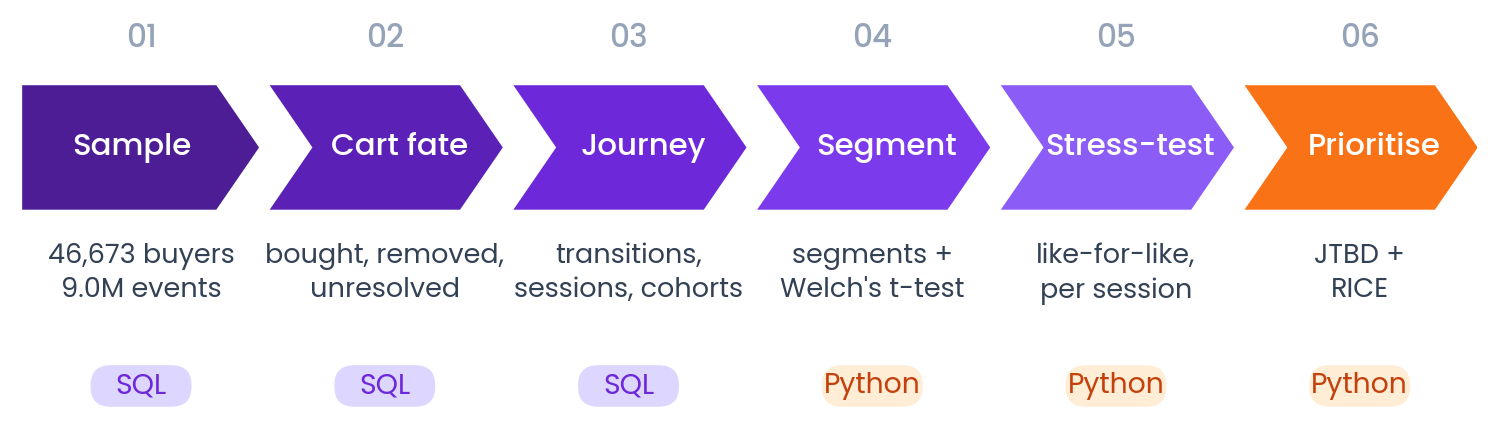
\includegraphics[width=0.95\linewidth]{fig00a_pipeline.png}
\caption{Analysis pipeline, from sampling to prioritisation.}
\label{fig:pipeline}
\end{figure}

\subsection{Metric framework: HEART}
Google's HEART framework~\cite{heart} organises user-experience metrics into Happiness, Engagement, Adoption, Retention and Task success, each broken into a goal, a signal and a metric. It was used to choose one metric for each dimension (Figure~\ref{fig:heart}). Task success is the core metric: the shopper's task is to buy what they put in the cart, so cart abandonment is task failure. Engagement is measured through sessions, searches and visits, and Retention through repeat purchases by cohort. The data has no ratings, surveys or feature launches, so Happiness and Adoption were measured through behavioural proxies. \emph{Happiness} is proxied by search success: of the sessions that include a search, the share that end with nothing carted or bought is treated as a frustration signal, with the share of cart items removed within ten minutes of being added (``cart regret'') as a second signal. \emph{Adoption} is proxied by feature uptake: the share of purchasers who have ever used the cart and the search function. These proxies describe behaviour consistent with satisfaction and uptake; they are not direct measures of either.

\begin{figure}[!htbp]
\centering
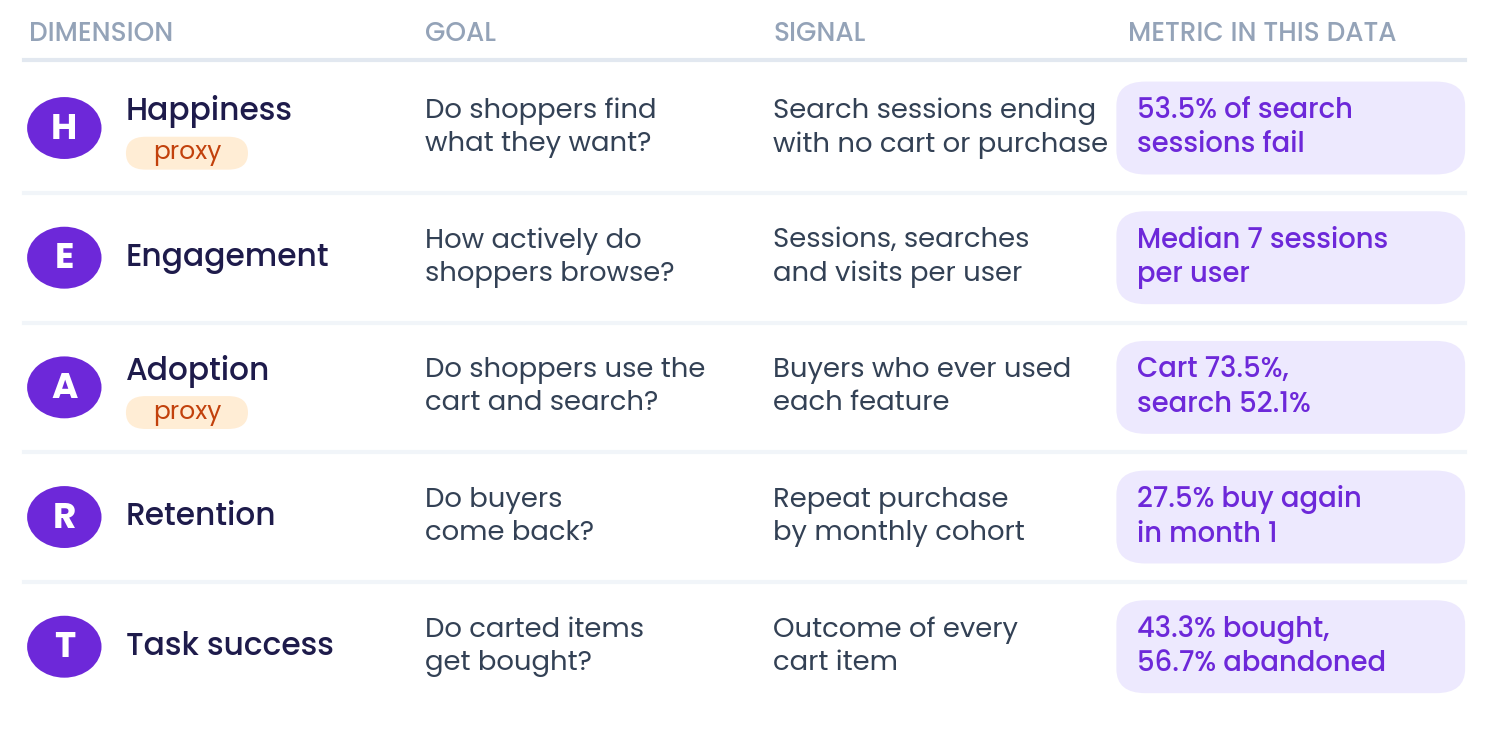
\includegraphics[width=\linewidth]{fig00b_heart.png}
\caption{HEART scorecard for this dataset: goal, signal and metric for each dimension. Happiness and Adoption are measured through behavioural proxies.}
\label{fig:heart}
\end{figure}

\subsection{Cart outcomes}
Each distinct (user, SKU) pair that was ever added to a cart is one \emph{cart item}, and has exactly one outcome: \emph{purchased} if the user bought that SKU, \emph{removed} if not bought but removed, and \emph{unresolved} otherwise. The abandonment rate is
\begin{equation}
\text{Abandonment} = \frac{\#\,\text{removed} + \#\,\text{unresolved}}{\#\,\text{cart items}} = 1 - \frac{\#\,\text{purchased}}{\#\,\text{cart items}}.
\end{equation}
Items carted just before the data ends have had little time to resolve, so the rate was recomputed excluding the last 14 days as a check on right-censoring.

\subsection{Journey, sessions and cohorts}
All events were combined into one time-ordered stream per user. The journey map is the row-normalised matrix of transitions from each event type to the next, computed with a \texttt{LEAD} window function. A session starts after 30 minutes without activity. Users were grouped into cohorts by the month of their first purchase in the window, and retention is the share of each cohort that buys again in later months.

\subsection{Segmentation and hypothesis testing}
For each user, the removal rate is removals divided by cart additions. Users were segmented as \emph{high-abandon} (removal rate $\geq 0.5$), \emph{moderate-abandon} ($0 <$ rate $< 0.5$) and \emph{low-abandon} (rate $= 0$), and by purchase frequency (one-time, repeat, five or more purchases). Search and visit counts were compared with Welch's t-test~\cite{welch}, which does not assume equal variances or equal group sizes; both apply here, since the groups differ several-fold in size and spread:
\begin{equation}
t = \frac{\bar{x}_{\text{high}} - \bar{x}_{\text{low}}}{\sqrt{s^2_{\text{high}}/n_{\text{high}} + s^2_{\text{low}}/n_{\text{low}}}}.
\end{equation}
Because the counts are heavily skewed, every comparison was repeated with the Mann--Whitney U test~\cite{mannwhitney} and reported with medians.

\subsection{Stress test and substitution}
\label{sec:stressmethod}
To check whether the headline comparison is fair, it was re-run on users with at least three cart additions only, comparing a high-removal group (rate $\geq 0.5$) with a low-removal group (rate $< 0.2$), first on totals and then per session. As a direct test of comparison shopping, each abandoned item was checked for a purchase of a \emph{different} SKU from the \emph{same} category by the same user within seven days of the cart addition.

\subsection{Price, category and prioritisation}
Purchase rates were compared across price quartiles using the correlation between price bucket and abandonment and a chi-square test with Cram\'er's $V$ as the effect size. Category abandonment was computed for the 465 categories with at least 200 cart items. Interventions were framed with Jobs-to-be-Done~\cite{jtbd} and ranked with RICE~\cite{rice}: $\text{RICE} = \text{Reach} \times \text{Impact} \times \text{Confidence} \,/\, \text{Effort}$, each scored on a 1--10 scale.

% =====================================================================
\section{Results}
\subsection{The user journey}
Figure~\ref{fig:overview} shows the scale of each event type and how many users reach each stage. Page visits make up three-quarters of all events. Just over half of purchasers ever searched, and about three in four used the cart. Purchase is 100\% by construction of the sample.

\begin{figure}[!htbp]
\centering
\placefig[0.95\linewidth]{fig01_data_overview.pdf}
\caption{(a) Number of events by type (log scale). (b) Share of the 46,673 users with at least one event of each type.}
\label{fig:overview}
\end{figure}

Figure~\ref{fig:journey} maps what shoppers do next, as the share of transitions from each event type to the next. Browsing dominates: 81\% of page visits lead to another visit, and 75\% of searches lead to a visit. The cart row is the most telling. After adding an item, the next action is a purchase only 3.2\% of the time; far more often the shopper goes back to browsing (59.0\%), adds another item (21.6\%) or searches again (8.5\%). Carting is part of the browsing loop, not its end point. Removals cluster (48.9\% of removals are followed by another removal), consistent with shoppers clearing out options once they have decided. Of all purchases, 77.3\% were of a SKU the user had carted beforehand, so the cart is the main path to purchase. In HEART terms, feature adoption among purchasers is high for the cart (73.5\%) and moderate for search (52.1\%).

\begin{figure}[!htbp]
\centering
\placefig[0.95\linewidth]{fig02_journey_transitions.pdf}
\caption{Journey map: for each event type, the share of transitions to each possible next event.}
\label{fig:journey}
\end{figure}

\subsection{Cart abandonment}
Of 450,463 cart items, 43.3\% were purchased, 40.5\% removed and 16.2\% left unresolved, an abandonment rate of \textbf{56.7\%} (Figure~\ref{fig:cart}a). Unresolved items are over-represented among the most recent cart additions, which is expected, but excluding the final 14 days changes the rate only to 56.2\%. When a carted item does sell, it usually sells fast: the median time from first cart-add to purchase is about 20 minutes, two-thirds of purchases happen within an hour, and 90\% within three days (Figure~\ref{fig:cart}b). An item still in the cart after a few days is unlikely to be bought.

The two Happiness proxies point the same way. Of 200,587 sessions that include a search, 53.5\% end with nothing carted or bought, so more than half of searches do not lead the shopper to something they want to keep. And 13.0\% of cart items are removed within ten minutes of being added, a quick change of mind that fits shoppers trying options out before committing.

\begin{figure}[!htbp]
\centering
\placefig[0.95\linewidth]{fig03_cart_outcomes.pdf}
\caption{(a) Outcome of every cart item; each square is 1\% of cart items. (b) Time from first cart-add to purchase, for items that were eventually bought.}
\label{fig:cart}
\end{figure}

\subsection{Cohorts}
Figure~\ref{fig:cohorts}a tracks each monthly cohort's repeat purchasing. For the July--October cohorts, 25--29\% buy again in the following month (27.5\% on average), and the curve stays flat after that: customers who return in month one tend to keep returning. The June cohort looks stronger because the window starts on 23 June, so it includes established customers whose true first purchase was earlier. Abandonment is almost identical across cohorts, between 52\% and 59\% (Figure~\ref{fig:cohorts}b), so it is not a problem of new or inexperienced customers. Over the whole window, 78.8\% of users bought more than once.

\begin{figure}[!htbp]
\centering
\placefig[0.95\linewidth]{fig04_cohorts.pdf}
\caption{(a) Share of each first-purchase cohort buying again $k$ months later; dotted segments end in December, which has only 8 days of data. (b) Cart abandonment rate by cohort.}
\label{fig:cohorts}
\end{figure}

\subsection{Who abandons: the headline comparison}
Table~\ref{tab:segments} and Figure~\ref{fig:segments} compare the abandonment segments. High-abandon users average 39.7 searches against 2.1 for low-abandon users, \textbf{18.9 times more}, and 276.8 page visits against 26.7, 10.4 times more. Both differences are highly significant under Welch's t-test ($t = 36.3$ and $43.6$, $p < 0.001$) and under Mann--Whitney.

\begin{table}[!htbp]
\centering\small
\caption{Abandonment segments (all 46,673 users)}
\label{tab:segments}
\begin{tabular}{lrrrrr}
\toprule
\textbf{Segment} & \textbf{Users} & \textbf{Searches} & \textbf{Visits} & \textbf{Cart adds} & \textbf{Never carted} \\
 & & \textit{(mean)} & \textit{(mean)} & \textit{(mean)} & \\
\midrule
Low abandon (rate $= 0$) & 24,355 & 2.1 & 26.7 & 1.3 & 50.7\% \\
Moderate abandon & 12,038 & 38.5 & 278.8 & 25.8 & 0\% \\
High abandon (rate $\geq 0.5$) & 10,280 & 39.7 & 276.8 & 28.6 & 0\% \\
\bottomrule
\end{tabular}
\end{table}

\begin{figure}[!htbp]
\centering
\placefig[0.95\linewidth]{fig05_segments.pdf}
\caption{Distribution of searches (a) and page visits (b) per user by abandonment segment, on a log scale. Boxes show the interquartile range, whiskers the 5th--95th percentiles and diamonds the mean.}
\label{fig:segments}
\end{figure}

Two details in the table matter. Half of the low-abandon group never added anything to a cart, and the moderate and high segments search almost identically (38.5 against 39.7). If searching drove abandonment, the high group should search clearly more than the moderate group. Both point to the same possibility: the 18.9$\times$ gap may mostly separate people who use the cart from people who don't.

\subsection{Stress-testing the headline}
\label{sec:stress}
Restricting the comparison to users with at least three cart additions removes non-cart users from both sides (8,404 high-removal and 6,358 low-removal users). Table~\ref{tab:stress} and Figure~\ref{fig:stress} show the result. High-removal users still search more in total, 2.3 times as much, with medians of 16 against 7. But they are also more active overall: 1.7 times more sessions and 2.5 times more cart additions. Per session, the difference in searching nearly disappears on average (1.36 against 1.28, a ratio of 1.07, $p = 0.047$), although the typical high-removal user still searches somewhat more per session (median 0.75 against 0.50, Mann--Whitney $p < 0.001$). Page visits per session do not differ in any meaningful way.

\begin{table}[!htbp]
\centering\small
\caption{Like-for-like comparison: users with 3+ cart additions (high removal $\geq 0.5$ vs.\ low removal $< 0.2$)}
\label{tab:stress}
\begin{tabular}{lrrrrl}
\toprule
\textbf{Measure} & \textbf{High} & \textbf{Low} & \textbf{Ratio} & \textbf{Medians} & \textbf{Welch $p$} \\
\midrule
Searches (total) & 47.9 & 20.7 & 2.32 & 16 vs 7 & $<0.001$ \\
Page visits (total) & 328.5 & 170.8 & 1.92 & 148 vs 86 & $<0.001$ \\
Sessions & 36.3 & 21.3 & 1.71 & 23 vs 13 & $<0.001$ \\
Cart additions & 34.6 & 13.7 & 2.53 & 14 vs 7 & $<0.001$ \\
Searches per session & 1.36 & 1.28 & 1.07 & 0.75 vs 0.50 & 0.047 \\
Visits per session & 9.90 & 10.37 & 0.95 & 6.4 vs 6.5 & 0.043 \\
\bottomrule
\end{tabular}
\end{table}

\begin{figure}[!htbp]
\centering
\placefig[0.9\linewidth]{fig06_stress_test.pdf}
\caption{Ratio of high- to low-abandon searches as the comparison becomes like-for-like (log scale).}
\label{fig:stress}
\end{figure}

The honest reading is that heavy abandoners are, above all, heavy users. They visit more often, cart more and search more, and within that they lean slightly towards searching. The 18.9$\times$ figure is a correct description of the segments, but most of it reflects cart usage rather than a distinct search behaviour.

\subsection{Direct evidence of comparison shopping}
The substitution test asks the comparison-shopping question more directly. Of 255,277 abandoned cart items, \textbf{21.0\%} were followed within seven days by the same user buying a different product from the same category, and 56.4\% by some purchase (Figure~\ref{fig:subst}). For heavy cart users the same-category rate is 20--23\%, against 12.5\% for the few items abandoned by low-abandon users. For roughly one abandoned item in five, the shopper evidently chose an alternative rather than walking away. That is a sizeable, well-defined group for a comparison feature to serve, and a more defensible basis for it than the raw search ratio.

\begin{figure}[!htbp]
\centering
\placefig[0.95\linewidth]{fig07_substitution.pdf}
\caption{What happened in the seven days after an item was abandoned: a purchase of a different SKU from the same category, some other purchase, or no purchase.}
\label{fig:subst}
\end{figure}

\subsection{Price and category}
Price does not explain abandonment. Purchase rates are nearly flat across price quartiles, from 45.3\% in the cheapest quartile to 42.3\% in the most expensive (Figure~\ref{fig:pricecat}a), and the correlation between price bucket and abandonment is 0.03. The chi-square test is significant only because of the sample size ($n = 450{,}463$); the effect size, Cram\'er's $V = 0.024$, is negligible.

Category matters more, but less than the extremes suggest. Across 465 categories, abandonment ranges from 28.5\% to 85.2\%, roughly a threefold spread. Half of all categories, however, fall between 51.6\% and 61.9\%, and only the tails of the ranked curve move far from the median (Figure~\ref{fig:pricecat}b), so the problem is broad rather than concentrated in a few categories. The outlying categories are worth a closer look, but because category IDs are anonymised, the data cannot say what they are.

\begin{figure}[!htbp]
\centering
\begin{minipage}[b]{0.44\textwidth}\centering\placefig{fig08_price.pdf}\end{minipage}\hfill
\begin{minipage}[b]{0.53\textwidth}\centering\placefig{fig09_categories.pdf}\end{minipage}
\caption{(a, left) Purchase rate by price quartile with 95\% confidence intervals; the dashed line is the overall rate. (b, right) The 465 categories ranked by abandonment rate; the shaded band is the middle half.}
\label{fig:pricecat}
\end{figure}

% =====================================================================
\section{From Insight to Intervention}
Each candidate intervention was framed as the job a shopper is trying to get done, then scored with RICE (Table~\ref{tab:rice}, Figure~\ref{fig:rice}). The scores are judgement-based estimates informed by the analysis, not measured quantities.

\begin{table}[!htbp]
\centering\small
\caption{Interventions framed with JTBD and ranked with RICE}
\label{tab:rice}
\begin{tabularx}{\textwidth}{>{\raggedright\arraybackslash}p{4.1cm}X cccc r}
\toprule
\textbf{Intervention} & \textbf{Job to be done} & \textbf{R} & \textbf{I} & \textbf{C} & \textbf{E} & \textbf{Score} \\
\midrule
Comparison tool for heavy searchers & ``Help me compare options quickly so I can decide with confidence'' & 8 & 8 & 7 & 5 & 89.6 \\
Reminders for items left in the cart & ``Remind me about items I was seriously considering'' & 6 & 7 & 6 & 3 & 84.0 \\
Better product info in high-abandon categories & ``Give me what I need to decide without leaving the cart'' & 5 & 8 & 6 & 6 & 40.0 \\
Personalised recommendations before cart-add & ``Show me relevant options without extensive searching'' & 9 & 6 & 5 & 7 & 38.6 \\
\bottomrule
\end{tabularx}
\end{table}

\begin{figure}[!htbp]
\centering
\placefig[0.92\linewidth]{fig10_rice.pdf}
\caption{RICE prioritisation: value (Reach $\times$ Impact $\times$ Confidence) against effort. Bubble size and label show the RICE score.}
\label{fig:rice}
\end{figure}

The comparison tool ranks first, but only narrowly ahead of cart reminders, which are much cheaper to build. The stress test argues for a measured rollout: the evidence supports comparison behaviour for about a fifth of abandoned items, not for all heavy searchers. A sensible plan is to ship reminders first as a quick win and test the comparison tool with a controlled experiment:
\begin{itemize}
  \item \textbf{Target:} users with several cart additions in a category within one session.
  \item \textbf{Randomisation unit:} user, so each shopper sees a consistent experience.
  \item \textbf{Primary metric:} cart-to-purchase rate for carted items (the task-success metric).
  \item \textbf{Guardrails:} average order value, return rate and page load time.
  \item \textbf{Success signal:} fewer items abandoned and then substituted within the same category.
\end{itemize}

% =====================================================================
\section{Limitations and Future Work}
\begin{itemize}
  \item \textbf{Purchasers only.} Sampling from the purchase log means the findings describe abandonment among customers who buy, not the whole visitor base, and no site-wide conversion rate can be computed.
  \item \textbf{Anonymised fields.} Prices are buckets, categories are IDs and search queries are embeddings, so the analysis cannot say which products or searches are involved.
  \item \textbf{Observational data.} The segment differences and the substitution pattern are associations. Only an experiment can show that a comparison tool would reduce abandonment.
  \item \textbf{Sample reproducibility.} The client sample was drawn without a fixed random seed. Re-sampling would give very close but not identical numbers.
  \item \textbf{Proxy metrics.} Happiness and Adoption are inferred from behaviour (search success, quick removals, feature use) because the data has no surveys or feature launches. A satisfaction survey or an actual feature release would measure them directly.
  \item \textbf{Window effects.} Items carted near the end of the window and the partial first and last months affect the unresolved share and the cohort edges; both are flagged where they matter.
\end{itemize}
Natural next steps are a random sample of all visitors to measure a true conversion funnel, sessionised funnels that follow a single shopping mission from search to purchase, and a controlled test of the top-ranked intervention.

% =====================================================================
\section{Conclusion}
More than half of all carted items (56.7\%) were never bought, and the rate is stable across cohorts and price levels. Mapping the journey shows that carting sits inside a browsing loop: a cart addition is followed by a purchase only 3\% of the time. Heavy abandoners search 18.9 times more than light abandoners, but a like-for-like comparison shows most of that gap reflects overall activity; per session the difference is small. The clearest evidence of comparison shopping is that one in five abandoned items is replaced by a same-category purchase within a week. Price plays almost no role. The recommendation is to ship low-effort cart reminders first and to test a comparison-shopping experience for heavy cart users in a controlled experiment, judged on the cart-to-purchase rate.

\section*{Tools and Environment}
\begin{itemize}
  \item \textbf{SQL:} DuckDB, for loading, de-duplication, cart-outcome tracking, \texttt{LAG}/\texttt{LEAD} window functions, sessionisation, cohort tables and \texttt{NTILE} segmentation.
  \item \textbf{Python:} pandas, NumPy, SciPy (Welch's t-test, Mann--Whitney U, chi-square, Spearman), matplotlib.
  \item \textbf{Frameworks:} HEART for metric selection, Jobs-to-be-Done for framing, RICE for prioritisation.
\end{itemize}

\begin{thebibliography}{9}
\bibitem{baymard} Baymard Institute. \textit{Cart \& Checkout Usability Research: Cart Abandonment Rate Statistics}. \url{https://baymard.com/lists/cart-abandonment-rate}
\bibitem{synerise} Synerise. \textit{RecSys Challenge 2025: Universal Behavioral Modeling}. \url{https://github.com/Synerise/recsys2025}
\bibitem{heart} K.~Rodden, H.~Hutchinson and X.~Fu (2010). Measuring the user experience on a large scale: user-centered metrics for web applications. \textit{Proceedings of the SIGCHI Conference on Human Factors in Computing Systems (CHI)}, 2395--2398.
\bibitem{welch} B.~L.~Welch (1947). The generalization of ``Student's'' problem when several different population variances are involved. \textit{Biometrika}, 34(1--2), 28--35.
\bibitem{mannwhitney} H.~B.~Mann and D.~R.~Whitney (1947). On a test of whether one of two random variables is stochastically larger than the other. \textit{Annals of Mathematical Statistics}, 18(1), 50--60.
\bibitem{jtbd} C.~M.~Christensen, T.~Hall, K.~Dillon and D.~S.~Duncan (2016). Know your customers' ``jobs to be done''. \textit{Harvard Business Review}, 94(9), 54--62.
\bibitem{rice} S.~McBride (2016). \textit{RICE: Simple prioritization for product managers}. Intercom. \url{https://www.intercom.com/blog/rice-simple-prioritization-for-product-managers/}
\bibitem{duckdb} M.~Raasveldt and H.~M\"uhleisen (2019). DuckDB: an embeddable analytical database. \textit{Proceedings of the 2019 International Conference on Management of Data (SIGMOD)}, 1981--1984.
\end{thebibliography}

\end{document}
